\chapter{Einleitung}
\label{chap:introduction}

%%%%%%%%%%%%%%%%%%%%%%%%%%%%%%%%%%%%%%%%%%%%%%%%%%%%%%%%%%%%
\section{Motivation}
\label{sec:introduction:motivation}
%%%%%%%%%%%%%%%%%%%%%%%%%%%%%%%%%%%%%%%%%%%%%%%%%%%%%%%%%%%%

Die GPS-Navigation ist seit Jahren aus keinem Auto mehr wegzudenken. Wo früher Karten genutzt wurden und nach Straßennamen geschaut wurde, wird heute die Zieladresse in das Navigationssystem eingegeben und das System bestimmt selbstständig die aktuelle Position, die Zielposition und errechnet die bestmögliche Route.
Ein Problem der GPS-Navigation ist jedoch, dass diese nur unter freiem Himmel akzeptabel funktioniert.
In der Realität verbringen wird jedoch den Großteil unserer Zeit in Gebäuden, wo uns dieser Ansatz wenig weiterhilft. 

Daher wäre es sinnvoll, eine Alternative zu GPS zu schaffen, welche diese Funktionien in Innenräume realisiert.
Da man jedoch für Innenräume kein eigenes Navigationssystem kaufen möchte, liegt die Idee nah, diese Konzept auf einem Gerät zu realisieren, was sowieso schon viele Leute besitzen und auch schon für die GPS-Navigation nutzen. 
Das Smartphone.
Wie in Abbildung 1 zu sehen, hat die Verbreitung der Smarthphones in den letzten Jahren sehr stark zugenommen, sodass man annehmen kann, das ein Großteil der potentiellen Nutzer der Indoor Positionierung auch ein Smartphone besitzt.
\begin{figure}[htb]
	\centering
		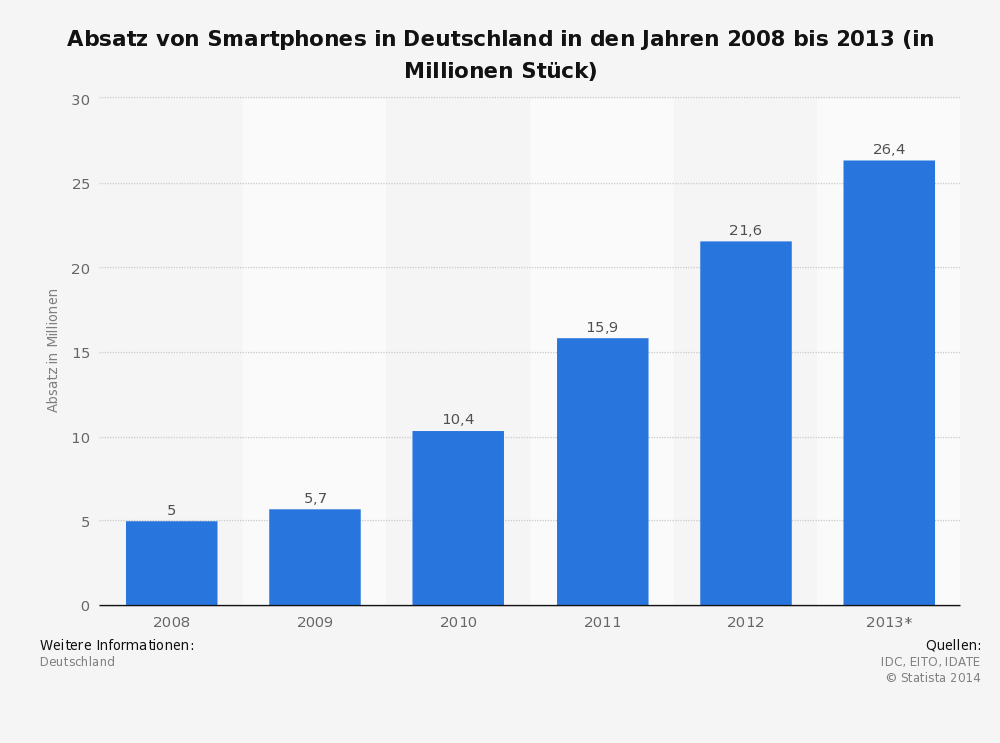
\includegraphics[height=8cm]{pictures/statistik-smartphonenutzung.png}
		\caption{Smartphoneabsatz in Deutschland}
\end{figure}

Für die Indoor Positionierung würden verschiedene Technologien in Frage kommen, wie zum Beispiel Wireless LAN, RFID oder Bluetooth.
Diese Technologien bieten sich an, da sie schon von Haus aus in vielen Smartphones integriert sind und so kein Bedarf an neuen Geräten oder Erweiterungen besteht.



Schlussendlich viel die Entscheidung der zu verwendenden Technologie auf Bluetooth, da dieses die höchste Verbreitung bietet und auch weitere Vorteile mit sich bringt. Zum einen ermöglicht Bluetooth eine schnelle und einfache Einrichtung und zum anderen benötigen die Bluetooth-Sendestationen nicht zwingend einen Stromanschluss, sondern erlauben auch einen Batteriebetrieb über mehrere Monate bis Jahre.

Die Positionierung in Innenräumen mittels Bluetooth ist ein relativ neuer Ansatz, welcher jedoch seit der Präsentation von Bluetooth Low Energy und der Vorstellung der iBeacons-Technologie von Apple immer mehr an Aufmerksamkeit gewonnen hat. 

%%%%%%%%%%%%%%%%%%%%%%%%%%%%%%%%%%%%%%%%%%%%%%%%%%%%%%%%%%%%
\section{Ziele der Bachelorarbeit}
\label{sec:introduction:goal}
%%%%%%%%%%%%%%%%%%%%%%%%%%%%%%%%%%%%%%%%%%%%%%%%%%%%%%%%%%%%


Das Hauptziel dieser Arbeit ist es zu untersuchen, in wie weit sich Bluetooth Low Energy beziehungsweise die darauf basierende iBeacons-Technologie für eine akzeptable Indoor Positionierung eignet, um Endgeräte zum Beispiel in Verkaufsräumen zu orten und zu identifizieren.

Dabei soll untersucht werden, welches Verfahren sich dafür am Besten eignet und ob es Unterschiede zwischen verschiedenen Sende- und auch Empfangsgeräten gibt.
Für die initialen Tests werden ausschließlich Apple-Geräte genutzt, da hier eine übersichtlichere Auswahl auf dem Markt ist, sodass man sich nicht mit unzähligen verschiedenen Messungen ausseinander setzen muss. 

Im Laufe der Bachelorarbeit soll deshalb eine iOS-Applikation entwickelt werden, welche eine Positionierung in einem Innenraum implementiert. Dabei wird die von Apple bereitgestellte CoreLocation-API genutzt, welche die Verarbeitung der iBeacon-Daten übernimmt. Die genutzten iBeacon-Sender kommen von Drittherstellern und sind derzeit noch in einem Vorserienstadium. 

Zum Abschluss soll eine grundlegende Positionierung, eine Anzeige der aktuellen Position auf eine Karte und das Auslösen bestimmter Aktionen an festgelegten Orten implementiert sein.



